% VECLYS Postprocessor -- the manual. Build with: make -C doc
\documentclass[11pt,a4paper]{article}

\usepackage[T1]{fontenc}
\usepackage{lmodern}
\usepackage{amsmath}
\usepackage{microtype}
\usepackage[margin=27mm]{geometry}
\usepackage{graphicx}
\usepackage{booktabs}
\usepackage{array}
\usepackage{longtable}
\usepackage{xcolor}
\usepackage{listings}
\usepackage{enumitem}
\usepackage[font=small,labelfont=bf]{caption}
\usepackage{parskip}
\usepackage[hidelinks]{hyperref}
\hypersetup{pdftitle={VECLYS Postprocessor User Guide},pdfauthor={}}

\definecolor{shell}{gray}{0.96}
\definecolor{comment}{rgb}{0.35,0.45,0.35}
\lstset{
  basicstyle=\ttfamily\small,
  backgroundcolor=\color{shell},
  commentstyle=\color{comment}\itshape,
  breaklines=true, columns=fullflexible, keepspaces=true, frame=none,
  xleftmargin=6pt, framexleftmargin=6pt, framexrightmargin=6pt,
  framextopmargin=4pt, framexbottommargin=4pt,
  aboveskip=\medskipamount, belowskip=\medskipamount,
}
\lstdefinestyle{sh}{language=bash}
\lstdefinestyle{py}{language=Python, keywordstyle=\color{blue!55!black}}
\lstdefinestyle{plain}{}

\newcommand{\prop}[1]{\textbf{#1}}          % a control in the Properties panel
\newcommand{\menu}[1]{\textbf{#1}}          % a menu item or a button
\newcolumntype{L}[1]{>{\raggedright\arraybackslash}p{#1}}

\title{\textbf{VECLYS Postprocessor}\\[2mm]
  \large User guide}
\author{}
\date{Initial release}

\begin{document}
\maketitle

\begin{abstract}
\noindent
Python plugins and toolbar buttons for working with a VECLYS case in ParaView:
open a run by the file that describes it, repeat one blade passage into a wheel,
work out the quantities the solver did not write, profile a slice from hub to
casing, and integrate one down to a row of numbers. Nothing here changes or
rebuilds ParaView --- it is a directory of Python files and a launcher. This
guide covers installing it and using it.
\end{abstract}

% Sections only: the subsections are many and short, and a contents that
% spills onto a second page for the sake of them is worse than none of them.
\setcounter{tocdepth}{1}
\tableofcontents
\clearpage

\section{What this is}

A turbomachinery CGNS file holds one blade passage, split into volume zones with
named boundary patches --- \path{BLADE}, \path{HUB}, \path{CASING},
\path{LEFT} and \path{RIGHT}. ParaView's own CGNS reader gives you the zones and
leaves the patches to be dug out; a run of several blade rows gives you a
directory tree to hunt through before you can open anything at all.

Two readers and five filters address that:

\begin{description}[style=nextline,leftmargin=6mm]
  \item[CGNS (labeled boundaries)] one \path{.cgns} file as a single entry in
    the Pipeline Browser, whose volume zones and named boundaries are
    checkboxes.
  \item[Veclys Reader] a whole run, opened by the \path{input.au3x} that
    describes it rather than by finding the meshes it wrote.
  \item[Circumferential Copy, Linear Copy] one passage repeated into a sector or
    a full wheel, at the pitch the case file states.
  \item[Flow Properties] Q-criterion, $\lambda_2$, vorticity, helicity,
    divergence, numerical schlieren.
  \item[Radial Profile] a slice reduced to a hub-to-casing table and plotted.
  \item[Surface Average] a slice reduced to one row: area, mass flow, averages.
\end{description}

Each filter has a button on the \menu{Macros} toolbar that sets it up for the
data in front of it, so the ordinary case is one click. Two of the buttons apply
what they make --- \menu{Radial Profile} and \menu{Surface Average}, since a
table of a few dozen numbers exists to be looked at. The two that build geometry
leave the filter unapplied, so a half-million-cell volume is not repeated
thirty-six times before the numbers have been checked.

\begin{figure}[t]
  \centering
  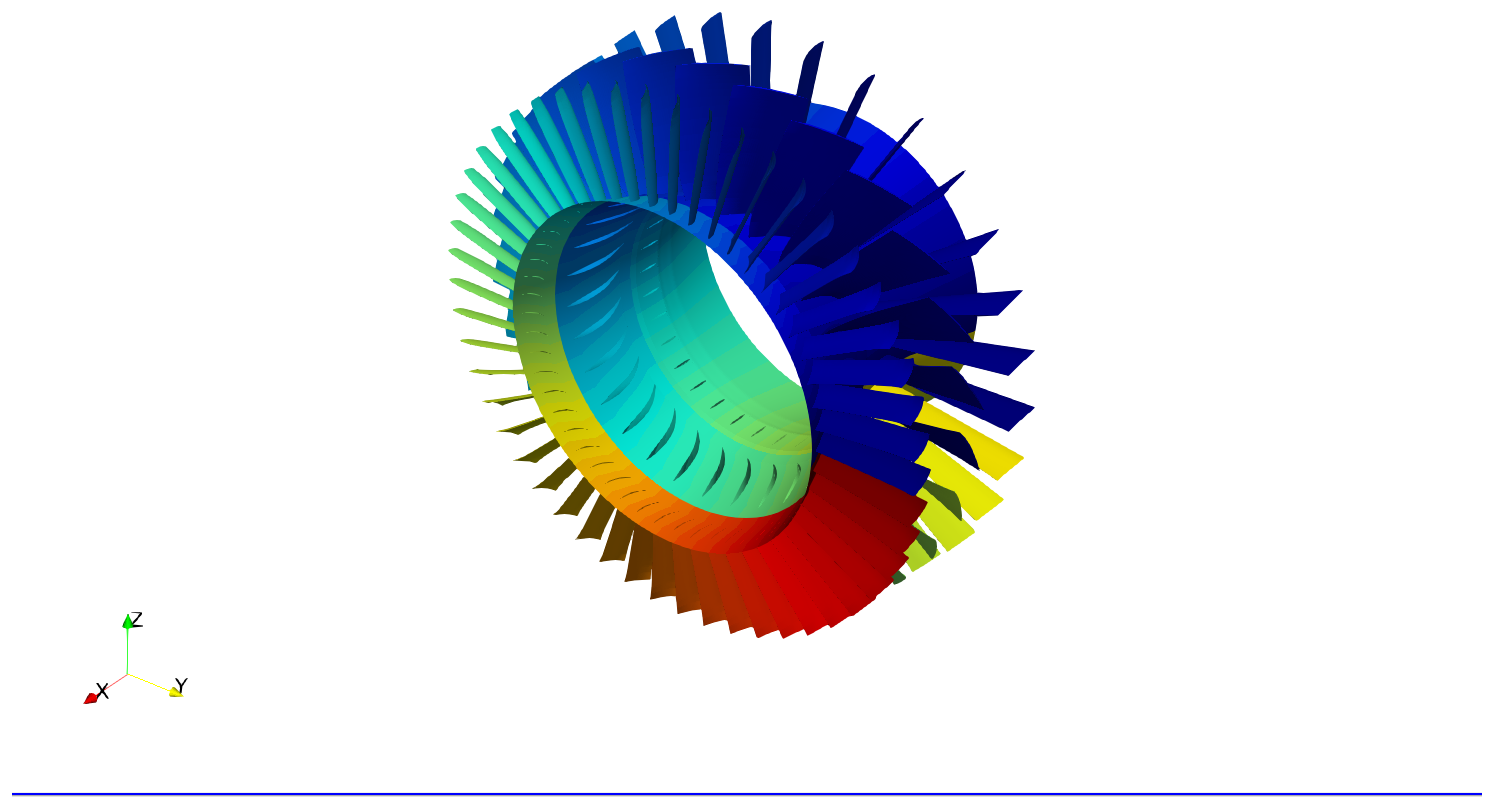
\includegraphics[width=\linewidth]{figures/annulus.png}
  \caption{A three-row stage closed into a full wheel by one filter. The rows
    have 32, 28 and 50 blades, so they are repeated 32, 28 and 50 times ---
    every one at its own pitch, read out of the run's \texttt{input.au3x}.
    Coloured by \texttt{CopyId}, which says which copy each blade is.}
  \label{fig:annulus}
\end{figure}

\section{Installing}

\subsection{What you need}

ParaView 6.1, and nothing else. It already carries everything the plugins import
--- \path{h5py} for reading CGNS section metadata, \path{numpy}, and the
\path{scipy} the verification suites use --- so there is no \path{pip} step and
nothing to build.

\path{zenity} is wanted by the buttons that ask for files: it is the desktop's
own file picker, and ParaView's Python has no Qt in it for a macro to open a
window with. Every mainstream Linux has it. Without it those buttons say so and
fall back to whatever is already selected.

\subsection{Running it}

Clone the repository anywhere and run the launcher. It takes the checkout to be
whatever directory it is sitting in, and finds ParaView through
\path{PARAVIEW_ROOT}, \path{PATH}, or common installation directories:

\begin{lstlisting}[style=sh]
git clone <this repo> ~/veclys_post
export PATH=~/ParaView-6.1.1-MPI-Linux-Python3.12-x86_64/bin:$PATH
~/veclys_post/paraview_diy.sh
\end{lstlisting}

The launcher does four things:

\begin{enumerate}[leftmargin=8mm]
  \item sets \path{PV_PLUGIN_PATH} to \path{plugins/}, which ParaView scans and
    auto-loads;
  \item puts \path{pylib/} on \path{PYTHONPATH} for the macros, which the
    plugins also do for themselves;
  \item links every file in \path{macros/} into
    \path{~/.config/ParaView/Macros}, which is what puts the buttons on the
    \menu{Macros} toolbar. The links point back at the repository, so editing a
    macro there is enough, and a file of the same name that is not a link is
    left alone;
  \item runs \path{auto_color_cgns.py} as a startup script, which picks the
    first coloring rather than leaving everything Solid Color.
\end{enumerate}

If the \menu{Macros} toolbar is not showing, \menu{View > Toolbars > Macros}
brings it back.

\subsection{Starting ParaView some other way}

\path{PV_PLUGIN_PATH} is read at startup, so a session begun from a desktop icon
or a plain \path{paraview} has none of the plugins, and the Open dialog has
never heard of \path{input.au3x}. ParaView's own answer is the \menu{Auto Load}
checkbox in \menu{Tools > Manage Plugins}, which it remembers in its settings
file. To tick them all at once, with ParaView closed:

\begin{lstlisting}[style=sh]
./install_autoload.py         # writes ~/.config/ParaView/ParaView.ini
./install_icons.py            # and gives each macro button its logo
\end{lstlisting}

Both keep a copy of the settings the first time, and both refuse to run while
ParaView is open, because ParaView writes the whole settings file out when it
closes and would undo the change. Both take \path{--settings} if your build
keeps its settings somewhere else.

\subsection{If ParaView will not start}

ParaView is an MPI build and carries its own MPI in \path{lib/}. A different MPI
on the environment --- the NVIDIA HPC SDK's, a Fluent or system one --- shadows
it, and the GUI aborts at startup with an \emph{Invalid communicator}
\path{MPI_Abort}. The launcher takes those off \path{PATH} and puts ParaView's
own \path{lib} first, so starting through it avoids the clash. Starting ParaView
any other way on such a machine will hit it.

\section{A worked session}

What follows is one pass through a stage, from the run directory to a number.
Each step is covered properly in its own section later.

\begin{enumerate}[leftmargin=8mm,itemsep=3pt]
  \item \textbf{Start it} with the launcher, so the plugins and the buttons are
    there.

  \item \textbf{Open the run.} \menu{File > Open}, and pick the
    \path{input.au3x} in the run directory --- not a mesh. The panel fills with
    the blade rows the case holds and the boundaries they carry. Tick the
    blades and click \menu{Apply}. One passage of each row appears.

  \item \textbf{Make a wheel.} With the reader selected, press
    \menu{Circumferential Copy}. The \prop{Blade Rows} table fills itself in
    from the case --- a line per row, with its blade count already there. Tick
    \prop{Full Annulus} and \menu{Apply}. Figure~\ref{fig:annulus} is the
    result.

  \item \textbf{Add what the solver did not write.} Select the reader again and
    press \menu{Flow Properties}. Choose the \prop{Velocity} array, leave
    \prop{Q-Criterion} ticked, \menu{Apply}. Then \menu{Filters > Contour} on
    it at a positive $Q$ to see the tip and passage vortices as surfaces.

  \item \textbf{Cut a station and profile it.} Select the reader and press
    \menu{Radial Profile}. It cuts a plane through the middle of the machine,
    profiles it, and opens a chart across the bottom of the window with the
    radius along the foot. Move the plane and press again for the next station:
    each gets a plot of its own, side by side.

  \item \textbf{Reduce it to numbers.} Select the slice and press \menu{Surface
    Average}. A SpreadSheet View opens under the render view with one row per
    block --- area, centre, and the area average of every property. Set
    \prop{Weighting} to \menu{Mass Flow Average} for the numbers that should be
    mass-averaged. The row is written to \menu{Output Messages} too.

  \item \textbf{Compare runs.} Export a profile or an average to CSV
    (\menu{File > Save Data}), then press \menu{Plot CSV Files} and pick the set
    --- this run's and the last one's --- to draw them on one chart.
\end{enumerate}

\section{Opening data}

\subsection{A CGNS file}

Open a \path{.cgns} file as usual. ParaView asks which reader to use, because
its own CGNS reader also claims the extension: choose \menu{CGNS (labeled
boundaries)}. Tick what you want and click \menu{Apply}.

\begin{center}
\begin{tabular}{@{}L{34mm}L{92mm}@{}}
\toprule
\prop{Volumes} & one checkbox per volume-bearing CGNS zone \\
\prop{Boundaries} & one checkbox per named boundary-face section --- the point
  of the reader: the patches are named in the file and are offered by those
  names \\
\prop{Cell Arrays}, \prop{Point Arrays} & the CGNS solution arrays, as usual \\
\prop{Cell Data to Point Data} & on by default; see below \\
\bottomrule
\end{tabular}
\end{center}

Unticking a boundary drops it from the output, and unticking everything in a
base means that base is never read at all. Only the section metadata is read
directly; the mesh and the solution arrays come from ParaView's own
\path{vtkCGNSReader}, driven from inside, so array naming and vector assembly
behave exactly as they do in the stock reader.

\prop{Cell Data to Point Data} is what makes contours and streamlines work
without a second filter: solvers write to cells, and most of ParaView's
interesting filters want points. Untick it when you want the solver's own cell
values --- for a threshold, or to see the discretisation as it is.

\subsection{A VECLYS case}

A run is a directory with an \path{input.au3x} in it, and the meshes are buried
a few folders down under names the input file only implies. Open the input file:

\begin{lstlisting}[style=plain]
File > Open > /path/to/run/input.au3x
\end{lstlisting}

The \path{[devicelist] device} line is the device tree --- comma-separated
chains, hyphens between the levels of a chain, each level written
\path{type:name}. Every device gets a folder of its own name, every device gets
a folder for the case number inside that, and the leaf writes its mesh there
under its own name. So

\begin{lstlisting}[style=plain]
device = empty:rotor37-dom:r37
\end{lstlisting}

with case 0000 is \path{rotor37/r37/0000/r37.cgns}, beside the input file. A case
of several blade rows lists them all,

\begin{lstlisting}[style=plain]
device = empty:e3-dom:IGV,empty:e3-dom:R1,empty:e3-dom:S1
\end{lstlisting}

and each becomes a block of the output, named after the row.

The panel is the CGNS reader's, over all the rows at once, plus:

\begin{center}
\begin{tabular}{@{}L{34mm}L{92mm}@{}}
\toprule
\prop{Domains} & one checkbox per blade row \\
\prop{Case Number} & the case the run wrote, which names the folder each mesh is
  in. Runs so far have only ever been case 0000 \\
\prop{Reload Case} & look for the case again. There is nothing else to press
  when a run writes its mesh after the case was opened: the panel has not
  changed, so ParaView has no reason to ask the reader anything \\
\bottomrule
\end{tabular}
\end{center}

A name carries its row's name only when more than one row uses it, so a stage's
three \path{HUB} patches are told apart while a lone one is not needlessly
qualified. Unticking a row leaves the names of the others --- and the ticks
against them --- where they were.

The rest of each \path{[<row>]} section is the run's own setup: the coordinate
system, the blade count, the shaft speed, the turbulence model. The copy button
reads three of those for you (section~\ref{sec:pitch}); the file itself is the
place to look for the others.

\subsection{What the blocks carry}

\begin{center}
\begin{tabular}{@{}L{34mm}L{92mm}@{}}
\toprule
\path{BoundaryId} & on every boundary block, for colouring or thresholding by
  boundary. Constant across a boundary, so it interpolates onto the points
  exactly along with everything else \\
\path{CGNSElementId} & the original 1-based CGNS element ID, only with
  \prop{Cell Data to Point Data} unticked --- an element id has no meaningful
  value at a point \\
\path{CGNSZoneName} & field data naming the zone the block was cut from \\
\bottomrule
\end{tabular}
\end{center}

\section{Repeating a passage}

A turbomachinery mesh holds one blade passage, so one passage is what the file
draws. \menu{Circumferential Copy} rotates copies of its input about the machine
axis and returns them as one multiblock. Press the \menu{Circumferential Copy}
button with a source selected, or pick the filter out of \menu{Filters >
Alphabetical}.

\subsection{The pitch comes from the case}
\label{sec:pitch}

\begin{figure}[t]
  \centering
  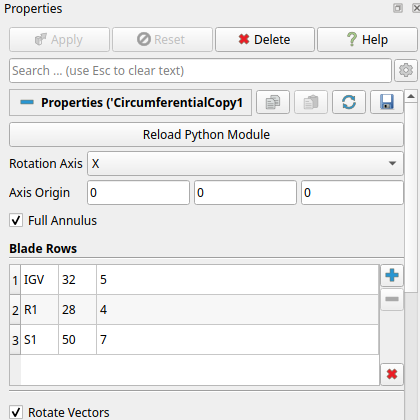
\includegraphics[width=0.55\linewidth]{figures/blade-rows.png}
  \caption{The panel after one press on a three-row stage. The names and blade
    counts came out of \texttt{input.au3x}; only the last column is worth
    touching, and \prop{Full Annulus} makes even that unnecessary.}
  \label{fig:panel}
\end{figure}

A blade count is a thing to look up, and looking it up is the part the case file
makes unnecessary: a run's \path{input.au3x} was written with the answer in it.
Press the button on anything built on a Veclys Reader and two keys of each
\path{[<row>]} section are read.

\path{cosystem} says whether there is an axis at all. \path{annular} is a machine
with one; \path{cartesian} is a straight cascade, which has none, and the button
makes a \menu{Linear Copy} for it instead (section~\ref{sec:linear}). This is
read \emph{first}, because a cartesian section keeps an
\path{assembly-sectors} that means nothing --- one test duct carries
\path{assembly-sectors=12} --- and taking that at face value would invent a
$30^\circ$ pitch for a mesh with no axis in it.

\path{assembly-sectors} is then the blade count of an annular row, and
\path{pitch} the passage spacing of a cartesian one.

The button also guesses the \textbf{machine axis} from a sample of a few
thousand of the input's points: a passage never crosses its own axis and covers
a narrow wedge about it, so the axis it stays clear of and looks narrowest from
is the one to pick. The guess and the wedge it measured go to the \menu{Output
Messages} window, as a warning when the answer is not clear-cut. A single blade
surface is genuinely ambiguous; a whole passage is not.

Pressed on a plain CGNS file there is no case to read: the axis is still
guessed, the settings of the last copy in the pipeline are inherited, and the
blade count is typed in once per session rather than once per boundary.

\subsection{The panel}

\begin{center}
\begin{tabular}{@{}L{34mm}L{92mm}@{}}
\toprule
\prop{Rotation Axis} & X, Y, Z, or \menu{Custom} with an \prop{Axis Direction}
  typed in \\
\prop{Axis Origin} & a point on the axis, which is 0 0 0 for the usual mesh \\
\prop{Full Annulus} & repeat every block its own blade count of times, whatever
  the copies column says \\
\prop{Blade Rows} & the table: a line per row, holding its name, its blade count
  and how many copies of it to make \\
\prop{Rotate Vectors} & on by default; see section~\ref{sec:vectors} \\
\bottomrule
\end{tabular}
\end{center}

\subsection{The Blade Rows table}

Everything about the copies is in that one table. A block the table names turns
by $360/\text{blades}$, that many times, and hands both down to everything under
it --- which is how one filter copies a whole stage with each row at its own
pitch, and why a stage stays a single entry in the Pipeline Browser. The button
fills it in, names and all, so nothing there has to be typed.

\begin{description}[style=nextline,leftmargin=6mm]
  \item[The line with no name] is what every other block goes by, which is all a
    mesh with no blade rows in it needs --- a plain CGNS file, a sphere. The
    filter starts with one such line, 36 blades and 4 copies.
  \item[An empty cell] keeps whatever that line says, so a line can set the
    copies alone.
  \item[A negative blade count] copies the other way round: $-48$ blades is a
    pitch of $-7.5^\circ$.
\end{description}

Anything the table cannot mean is refused by the line it is on --- two lines for
one row, a cell that is not a number, half a blade --- and nothing is drawn
rather than something wrong. A line naming a block the input has not got, and a
block the table leaves with no pitch, are reported by name in \menu{Output
Messages}; the block is copied once, where it is, rather than failing the
filter.

\subsection{Full annulus}

\prop{Full Annulus} is the usual answer and the one number nobody should have to
work out: rows of 32, 28 and 50 blades close the wheel together, at 32, 28 and
50 copies (figure~\ref{fig:annulus}).

Without it, the button starts each row on four copies of the widest-pitched
row's worth of machine --- so the rows line up, and \menu{Apply} does not build a
whole wheel by accident. A wheel of a large volume is a large thing: the copies
share their cells and arrays, but there is one set of coordinates per copy, so
check the counts before applying.

\subsection{What comes out}

Each dataset in the input is replaced by a multiblock of its copies, so the
input's own tree survives:

\begin{lstlisting}[style=plain]
Root
+- Boundaries
   +- BLADE_quad
      +- Copy 0        the input, where it already is
      +- Copy 1        one pitch on
      +- ...
\end{lstlisting}

Keeping the tree this way round means the Multi-block Inspector can still hide
\path{BLADE_quad} in every copy at once, and block paths gain a \path{/Copy 1}
on the end rather than changing shape.

\begin{center}
\begin{tabular}{@{}L{34mm}L{92mm}@{}}
\toprule
\path{CopyId} & which copy this is, constant across it. Put on whichever
  attribute the data already uses, so it is offered once in the colouring
  dropdown rather than twice \\
\path{CopyAngle} & field data: how far this copy was turned, in degrees \\
\path{CopyOffset} & the same for a \menu{Linear Copy}, in the mesh's own unit \\
\path{CopyId2}, \path{CopyAngle2} & a second round of copying --- a sector of
  three, then twelve of those --- labels alongside the first rather than over it \\
\bottomrule
\end{tabular}
\end{center}

Only the points of a copy are new. The cells and the arrays that were not
rotated are passed through by reference, so a full annulus costs one set of
coordinates per copy rather than one whole mesh.

\subsection{Rotating vectors}
\label{sec:vectors}

A velocity that was not turned with the geometry would point the wrong way in
every copy but the first, so \prop{Rotate Vectors} is on by default and turns
every three-component array of floats --- including the cell arrays, which is
what the reader produces with its \prop{Cell Data to Point Data} unticked.

Three-component arrays of any other type are left where they are. Only a
floating-point triple can hold a rotated vector: a colour stored as three
unsigned bytes would come back with its components mixed and then wrapped around
by its own type, so $(10, 20, 30)$ would turn into $(237, 10, 30)$.

Untick the box and nothing is touched at all --- including the array ParaView has
marked as the active vectors, which \path{vtkTransformFilter} would otherwise
rotate on its own. Either way the copies agree with the input about which array
is the active vectors, so ParaView's own filters downstream pick the same
default.

\subsection{From Python}

\begin{lstlisting}[style=py]
copies = CircumferentialCopy(Input=reader)
copies.RotationAxis = 'X'
copies.BladeRows = ['', '36', '4']   # no name: everything the input holds
copies.FullAnnulus = 1               # 36 copies, the whole wheel
\end{lstlisting}

The table is flat, three strings to a line:

\begin{lstlisting}[style=py]
copies.BladeRows = ['IGV', '32', '5',
                    'R1',  '28', '4',
                    'S1',  '50', '7']
\end{lstlisting}

\section{Repeating a cascade}
\label{sec:linear}

A linear cascade is the flat cousin of a blade row: the mesh holds one passage
and the machine is that passage translated over and over, with no axis anywhere.
VECLYS writes one whenever \path{input.au3x} says \path{cosystem=cartesian}, and
\menu{Linear Copy} is the filter for it. There is no separate button --- the
\menu{Circumferential Copy} button makes one of these when the case is
cartesian, and says so.

The file gives the distance between two passages and not which way they lie, so
the direction is \emph{measured off the mesh}: the two periodic patches,
\path{LEFT} and \path{RIGHT}, are one pitch apart by construction, so the vector
between their centroids is both the direction and a check on the number. Only
those two patches are read, which is a few hundred faces however big the volume
is. A mesh with no such pair is reported and the direction left for you to set;
so is a case file that gives no pitch, rather than one being invented.

The panel is the circumferential one with the rotation taken out:
\prop{Translation Direction}, and the same \prop{Blade Rows} table with the
distance between passages where the blade count would be. There is no
\prop{Full Annulus} --- a cascade is a straight line of passages with no wheel to
close, so how many of them to draw is the only answer there is. There is no
\prop{Rotate Vectors} either, because the question does not come up: sliding a
mesh sideways leaves every velocity pointing where it did.

\section{Derived quantities}

A CGNS file carries what the solver wrote and none of the quantities that come
from its derivatives. The \menu{Flow Properties} button adds those. It leaves the
filter unapplied, because working out derivatives over half a million cells is
not something to start by accident.

Two dropdowns say which arrays to work from: \prop{Velocity} lists the
three-component arrays in the input and \prop{Density} the single-component
ones, and nothing else is offered, so neither can be pointed at a pressure by
mistake.

\paragraph{The density is the one to watch.} A CGNS file often has no density in
it, and the \prop{Density} box then lands on whichever array comes first, which
is why the two quantities that read it start unticked. Make one first with a
\menu{Calculator}:

\begin{lstlisting}[style=plain]
Result Array Name:  Density
Expression:         Pressure/(287.058*Temperature)
\end{lstlisting}

That is the ideal gas law for air. It is worth having anyway: \menu{Surface
Average} wants a density too, for its mass-flow averaging.

The \prop{Quantities} list is a set of checkboxes. Only \prop{Q-Criterion} and
\prop{Vorticity Magnitude} start ticked, because they are what any velocity field
can give; everything else is opt-in.

\begin{center}
\begin{tabular}{@{}L{40mm}L{86mm}@{}}
\toprule
\prop{Q-Criterion} & $(\lVert W\rVert^2 - \lVert S\rVert^2)/2$, equivalently
  $-\tfrac{1}{2}\mathrm{tr}(G^2)$, where $G$ is the velocity gradient and $S$,
  $W$ its symmetric and antisymmetric halves. A vortex core is where it is
  positive \\
\prop{Lambda2} & the middle eigenvalue of $S^2 + W^2$; a core is where it is
  negative. Both are the standard definitions and both are transpose-invariant,
  so which way round the gradient is stored cannot change them \\
\prop{Vorticity}, \prop{Vorticity Magnitude} & the curl of the velocity, and how
  fast the fluid is spinning \\
\prop{Helicity} & velocity dotted with vorticity, which distinguishes a vortex
  the flow runs along from one it crosses \\
\prop{Divergence} & zero in an incompressible solution, so a map of it is a map
  of how well converged the continuity equation is \\
\prop{Density Gradient Magnitude} & the raw shock picture \\
\prop{Numerical Schlieren} & $\exp(-k\,|\nabla\rho| / \max|\nabla\rho|)$, white
  where the density is uniform and black across a shock, with \prop{Schlieren
  Exponent} as the $k$ that decides how hard it darkens \\
\bottomrule
\end{tabular}
\end{center}

Everything comes from one pass of \path{vtkGradientFilter} per mesh, so asking
for six quantities costs little more than asking for one, and each lands on the
same attribute --- points or cells --- as the velocity or density it came from.
A quantity whose source array is missing is reported by name rather than
silently skipped.

\section{Radial profiles of a slice}

The \menu{Radial Profile} button cuts a plane through the middle of the machine,
normal to the axis it guesses from the input's points, puts a \menu{Radial
Profile} on it, and opens a Line Chart View \emph{across the bottom of the
window} with the radius along the foot and the flow properties up the side.
Press it on a slice you have already placed and it profiles that one instead,
taking the machine axis from the plane's own normal.

The filter takes \prop{Number Of Bands} radii across the span and contours the
input at each. That curve is where the band cuts the slice, and every property on
it is averaged \emph{weighted by edge length}. It matters: the curve at mid-span
of a rotor can be a couple of hundred edges whose lengths span a factor of
several hundred, tightening where the mesh does against the blade, and a mean
over the points would count that crowd of short edges as if each carried a full
share of the circumference.

\begin{center}
\begin{tabular}{@{}L{40mm}L{86mm}@{}}
\toprule
\prop{Rotation Axis}, \prop{Axis Origin} & the machine axis. There is no guessing
  inside the filter: a planar slice looks narrow from any axis lying in it, so
  the axis is asked for rather than inferred \\
\prop{Number Of Bands} & 50 by default \\
\prop{Spacing} & \menu{Clustered at the walls} by default, which is where a
  turbomachine's gradients are --- the samples are the interior points of a
  cosine distribution, so the first sits a two-thousandth of the span from the
  hub rather than a hundredth. Switch to \menu{Uniform} if the rows are going to
  be averaged back into one number, since only then do they carry equal weight \\
\prop{Automatic Radius Range} & on by default, taking hub and casing from the
  input. Untick it to profile part of the span, or to hold the range still while
  comparing one slice with another \\
\bottomrule
\end{tabular}
\end{center}

The output is a table: one row per band, a \path{Radius} column, a \path{Length}
column for the curve the band cut, and one column per property. Bands that miss
the input are left out rather than filled with nothing, and how many were dropped
is reported.

\paragraph{One plot per station.} Pressing the button again gives the next
station a plot of its own beside the last, rather than drawing over it, so a run
of slices down the machine can be compared at a glance. Each plot is titled with
where its slice is, and the row is kept evenly wide however many there are. To
draw over the last plot instead, set \path{_A_PLOT_EACH = False} at the top of
\path{macros/Radial Profile.py}.

This matters because ParaView's own eye icon draws a source into whatever view is
\emph{active}, so making a profile visible from the Pipeline Browser drops it
onto whichever plot you last clicked. Closed a station's plot, or found one
crowding another's? Select that profile and press the button: it is moved to a
plot of its own, and the one it was crowding is left as it was.

Every property is drawn, less \path{Radius} and \path{Length}. They share one
left-hand axis, so a pressure of 130{,}000 flattens a temperature of 320 against
the floor: untick in \prop{Series} the ones you are not comparing.

\section{Integrating a slice}

The \menu{Surface Average} button reduces the selected slice to one row and opens
it in a SpreadSheet View across the bottom of the window. Pressing it again
reuses that view rather than carving the window up a second time. It also writes
the row to \menu{Output Messages}, which is quicker to read than a table when all
you wanted was the mass flow.

A multiblock input --- a slice of several zones, or a set of boundary patches ---
gives \emph{one row per block} by default, each named in the \path{Surface}
column by its path in the Multi-block Inspector, and a \path{Centre} column puts
it in space, which is how one axial station is told from another. \prop{Rows} set
to \menu{Everything Together} adds the blocks into a single row instead.

\begin{lstlisting}[style=plain]
Surface                 Area       Centre                    Pressure
Boundaries/HUB_quad     0.004655   (0.0324, 0.0020, 0.1827)   106850
Boundaries/CASING_quad  0.006485   (0.0324, 0.0019, 0.2456)   112020
\end{lstlisting}

\prop{Weighting} decides what the row holds:

\begin{center}
\begin{tabular}{@{}L{40mm}L{86mm}@{}}
\toprule
\menu{Integral} & the plain integral of each property over the surface \\
\menu{Area Average} & that divided by the area, which is the default. On a solid
  rather than a surface it is a volume average, and the first column says
  \path{Volume} rather than \path{Area} so the table cannot lie about it \\
\menu{Mass Flow Average} & each point weighted by the mass crossing the surface
  there, which is how a stagnation quantity should be averaged. It needs a
  \prop{Density} and a \prop{Velocity} array and adds a \path{MassFlow} column.
  The surface normal comes from the geometry, so the sign of the flux follows
  whichever way the normals happen to point; the mass flow is reported positive
  and the averages are unaffected, being ratios \\
\bottomrule
\end{tabular}
\end{center}

Both this and the radial profile integrate through \path{vtkIntegrateAttributes},
the same code behind ParaView's own \menu{Integrate Variables}, so every cell
counts for its own area and not for one cell's worth. Two triangles of area 0.5
and 50 carrying 1 and 100 average to 99.02, not to 50.5 --- and a slice of a
rotor is twelve thousand triangles whose areas span a factor of a thousand, so
the difference is not academic.

\section{Plotting CSV files}

The profile and the averages write CSV, and a rig or another run gives CSV, so
\menu{Plot CSV Files} opens several at once and draws them on one chart. Press
the button, pick the files of a set, and each is opened and plotted against its
own radius column --- found by name, or the first column if none matches --- with
its series named after the file, so \path{runA: Pressure} and
\path{runB: Pressure} are told apart in the legend. The charts open in a tab of
their own, named \emph{CSV Files}, so they never crowd the render view.

\paragraph{A plot per press.} Press again with another set and that set gets its
own chart beside the first, evenly wide, so several sets sit side by side. Each
chart is titled after the folder its set came out of; two sets out of one folder
are told apart by qualifying the title. Set \path{_A_PLOT_EACH = False} at the
top of the macro to go back to one chart, cleared and redrawn each press.

\paragraph{A file can go on as many charts as it belongs on.} Picking one that is
already open draws the source already there rather than opening the file again,
so it stays a single entry in the Pipeline Browser under the name it was given.
It is re-read as it is picked, since a file worth picking again is often one that
has been written again.

\section{Troubleshooting}

\begin{center}
\begin{longtable}{@{}L{52mm}L{74mm}@{}}
\toprule
\textbf{What you see} & \textbf{What to do} \\
\midrule
\endhead
ParaView aborts at startup with \emph{Invalid communicator} &
  Another MPI on \path{PATH} is shadowing ParaView's own. Start it through the
  launcher, which takes the foreign one off \\
\addlinespace
A button says the plugins are not loaded &
  ParaView was started some other way. Use the launcher, or run
  \path{install_autoload.py} once with ParaView closed \\
\addlinespace
The Open dialog has never heard of \path{input.au3x} &
  The same: the reader is a plugin, and plugins are found at startup \\
\addlinespace
ParaView asks which reader to use for a \path{.cgns} &
  Its own CGNS reader claims the extension too. Choose \menu{CGNS (labeled
  boundaries)} \\
\addlinespace
No file picker appears &
  \path{zenity} is not installed. Open the files yourself with \menu{File >
  Open}, select one, and press the button \\
\addlinespace
The machine axis was guessed wrong &
  Pressed on a single blade surface, which is genuinely ambiguous. Set
  \prop{Rotation Axis} by hand, or press on the whole passage \\
\addlinespace
The table names a row the input has not got &
  A row was extracted upstream, or a name was edited. The message says which
  name; delete that line or correct it \\
\addlinespace
Nothing is drawn and the table is complained about &
  Two lines for one row, a cell that is not a number, or half a blade. The
  message says which line \\
\addlinespace
A block came through uncopied &
  Nothing in the table gave it a pitch, and the line with no name on it was
  deleted. Put one back \\
\addlinespace
The shock picture is blank or wrong &
  \prop{Density Gradient Magnitude} and \prop{Numerical Schlieren} are the two
  quantities that read the \prop{Density} dropdown, and it lands on whatever
  single-component array came first. Make a real density with a
  \menu{Calculator} and choose it \\
\addlinespace
A profile plot is a flat line &
  One property's numbers dwarf the rest on the shared axis. Untick the others in
  \prop{Series} \\
\bottomrule
\end{longtable}
\end{center}

\section{Checking the installation}

Five verification suites run headless and check the answers against ones known
before the code runs. They are the quickest way to tell whether an installation
is sound:

\begin{lstlisting}[style=sh]
pvpython verify_plugin.py               path/to/a.cgns
pvpython verify_circumferential_copy.py path/to/a.cgns
pvpython verify_passage_copies.py       path/to/a.cgns
pvpython verify_veclys_reader.py        path/to/input.au3x
pvbatch --force-offscreen-rendering verify_flow_tools.py
\end{lstlisting}

They are worth more than a smoke test. The flow tools are checked against
answers arithmetic gives: a solid body turning at 2\,rad/s with a drift along
the axis has a vorticity of $(0,0,4)$, a $\lambda_2$ of $-4$, a $Q$ of 4 and no
divergence, and the filter gets every one of them exactly. The copies are checked
against the mesh itself: one pitch must carry the \path{LEFT} patch onto the
\path{RIGHT} one, which it does to within $2.6\times10^{-8}$ on a mesh 0.149
across.

Two things do not travel with the repository. The CGNS meshes are gitignored, so
the checks that default to \path{bfs.cgns} and \path{r37.cgns} want a file of
your own as their argument. Pass your own \path{input.au3x} files to
\path{verify_veclys_reader.py}, or set \path{PARAVIEW_DIY_CASES_DIR} to a
directory whose child folders contain those files. The default is
\path{TestCase/veclys} inside the checkout.
\path{verify_passage_copies.py} looks for reference cases in the \path{stage},
\path{wheel}, \path{cascade}, and \path{duct} child folders and reports missing
cases. Set \path{PARAVIEW_DIY_STAGE_CASE}, \path{PARAVIEW_DIY_WHEEL_CASE},
\path{PARAVIEW_DIY_CASCADE_CASE}, or \path{PARAVIEW_DIY_DUCT_CASE} to select
each reference \path{input.au3x} explicitly. The optional coloring check uses
\path{PARAVIEW_DIY_COLOR_CASE}.

\section{What is where}

\begin{center}
\begin{tabular}{@{}L{34mm}L{92mm}@{}}
\toprule
\path{plugins/} & one file per reader or filter; ParaView auto-loads the lot \\
\path{macros/} & one file per toolbar button, linked into ParaView's Macros \\
\path{pylib/} & what the plugins and the macros share \\
\path{icons/} & the toolbar logos \\
\path{doc/} & this manual \\
\path{verify_*.py} & the headless verification suites \\
\bottomrule
\end{tabular}
\end{center}

\path{pylib/} is the only place a macro and a plugin can meet: ParaView runs a
macro as a bare string with no \path{__file__} to find anything by, so the
plugins put \path{pylib/} on the path as they load and the launcher puts it on
\path{PYTHONPATH} as well. It holds \path{passage_copies.py} (the walk over the
input, the Blade Rows table and the labels, shared by the two copy filters),
\path{veclys_case.py} (what an \path{input.au3x} says, shared by the reader and
the copy button so the two cannot disagree about a file) and
\path{paraview_diy_macros.py} (what the buttons have in common).

The README in the repository root covers the same ground at greater length, with
the reasoning behind the choices and the measured numbers the verification
suites check against.

\end{document}
